\documentclass[12pt]{article}
\usepackage{graphicx}
\usepackage{psfrag}
\usepackage{epsfig}
\usepackage{subfigure}
\usepackage{amssymb,amsmath}
\usepackage{verbatim}

%\usepackage{doublespace}

\textheight 23cm \topmargin -1cm \leftmargin 0cm

\marginparwidth 0mm    % Largeur des notes marge de droite
\textwidth 16.5cm      % Largeur du texte
\hsize \textwidth      % Longueur d'une ligne
\advance \hsize by -\marginparwidth
\oddsidemargin -4mm    % Marge gauche pages de droite - 1 inch (2.54 cm)
\evensidemargin \oddsidemargin % Idem pour les pages de gauche

\advance\hoffset by 5mm % Pour corriger un decalage residuel sur la gauche

\renewcommand{\hat}{\widehat}
\newcommand{\R}{\mathrm{I\!R\!}}
\newcommand{\C}{\mathrm{I\!\!\!C\!}}
\newcommand{\sinc}{\mbox{sinc}}
\newcommand{\diag}{\mbox{diag}}
\newcommand{\Tr}{\mbox{Tr}}

% commands
\newtheorem{theo}{Theorem}
\newtheorem{proposition}{Proposition}
\newcommand{\nc}{\newcommand}
\nc{\RR}{\mbox{\rm I$\!$R}} \nc{\dsp}{\displaystyle}
\nc{\Div}{\mbox{\rm div }} \nc{\beequ}{\begin{equation}}
\nc{\barr}{\begin{array}} \nc{\earr}{\end{array}}
\nc{\eequ}{\end{equation}} \nc{\BFF}{\hbox{\boldmath{${\cal
F}$}}^{(j)}({\bf y}^s,t)}

\nc{\hr}{\widehat{r}} \nc{\hh}{\widehat{h}} \nc{\hs}{\widehat{s}}
\nc{\hn}{\widehat{n}} \nc{\hw}{\widehat{w}} \nc{\hd}{\widehat{d}}
\nc{\hG}{\widehat{\Gamma}} \nc{\om}{\omega} \nc{\yy}{{\bf y}}
\nc{\ys}{{\bf y}^s} \nc{\yo}{{\bf y}_0} \nc{\xp}{{\bf x}_p}
\nc{\xr}{{\bf x}_r} \nc{\co}{{\cal O}}
\renewcommand\labelenumi{\alph{enumi})}
\begin{document}
\begin{center}
\textbf{Practice Set 3 Solutions}
\end{center}
\paragraph{Problem 1}
%$${\bf G_{ZF}}=\sqrt{M_T}{\bf (H^HH)^{-1}H^H}$$
\begin{eqnarray*}
{\bf G_{ZF}} &=& \sqrt{M_T}{\bf (H^HH)^{-1}H^H}=\left[
\begin{array}{cccc}
-0.8787 - 1.3185j &  0.0132 + 1.1870j \\
-0.6193 - 0.0484i & 1.5225 + 0.3681i
\end{array}
\right]
\end{eqnarray*}

To verify this set ${\bf X}=[1 + j~~-1 + j]^T$, then ${\bf Y}=\sqrt(1/M_T){\bf HX}$
\begin{eqnarray*}
\hat{{\bf X}} &=& {\bf G_{ZF}Y}=\left[\begin{array}{cccc}
1 + j  \\
-1 + j 
\end{array}
\right]
\end{eqnarray*}
\paragraph{Problem 2} {\it Diversity Gain} 
\begin{enumerate}
\item
We can express the received signal model as
\begin{equation*}
{\bf y} = \sqrt{E_s} {\bf h} s + {\bf n}
\end{equation*}
With MRC,
$$
z  =  \sum_{i=1}^M h_i^* y_i  =   {\bf h}^H {\bf y}  = \sqrt{E_s} {\bf h}^H {\bf h}s + {\bf h}^H {\bf n}
$$
Signal Power
\begin{eqnarray*}
{\cal E}\left \{ \left [ \sqrt{E_s} {\bf h}^H {\bf h}s   \right] \left[ \sqrt{E_s} {\bf h}^H {\bf h}s \right] ^H \right \}
=E_s \left( \Vert  {\bf h} \Vert  ^2\right)^2 {\cal E} \{s s^*\} 
= E_s \left( \Vert  {\bf h} \Vert  ^2 \right)^2
\end{eqnarray*}
Noise Power
\begin{eqnarray*}
{\cal E} \left \{ \left [ {\bf h}^H {\bf n} \right]\left [ {\bf h}^H {\bf n} \right]^H \right \}= {\bf h}^H {\cal E} \{ {\bf n n}^H \} {\bf h}= {\bf h}^H ( N_0 {\bf I}) {\bf h} = N_0 \Vert h\Vert ^2
\end{eqnarray*}
SNR
\begin{eqnarray*}
\eta 
= \frac { E_s ( \Vert  {\bf h} \Vert  ^2)^2 } {N_0 \Vert h\Vert ^2} 
=  \Vert {\bf h}\Vert ^2 \rho 
\end{eqnarray*}

\item The processed signal is given by
\begin{eqnarray*}
{ z} & = & {\bf h}^H {\bf y}  = \sqrt{E_s} \Vert {\bf h}\Vert ^2 s + {\bf h}^H {\bf n}
\end{eqnarray*}
Dividing it by $ \sqrt{E_s} \Vert {\bf h}\Vert ^2$  does not change the decision at the receiver.
\begin{eqnarray*}
{\tilde z} &=& s + \frac{ {\bf h}^H {\bf n}  } { \sqrt{\frac{E_s}{M}} \Vert {\bf h}\Vert ^2 } \\
& \Rightarrow &  {\bf n}  \rightarrow {\cal N} ( 0, \frac{N_0}{ {E_s} \Vert  h\Vert ^2}) \rightarrow {\cal N} ( 0, \frac{1}{\eta})
\end{eqnarray*}
Using the Nearest Neighbor Union Bound (NNUB), the probability of symbol error $P_e$ is given as
\begin{equation*}
P_e \le {\overline N_e} Q \left[ \frac{d_{min}} {2 \sigma_n} \right]
\end{equation*}
where $d_{min}$ is the minimum distance between any two points in the constellation and $\sigma_n^2 = \frac {{\cal N}_0}{2} = \frac{1}{2 \eta}$ is the variance per dimension of the AWGN. $Q (\cdot )$ is the Q-function defined as
\begin{eqnarray*}
Q(x) =  \frac{1}{2 \pi} \int_x^\infty  e ^{\frac{-u^2}{2}} du
\end{eqnarray*}
$\overline N_e$ is the average number of nearest neighbors for the signal constellation.
The probability of symbol error becomes
\begin{eqnarray*}
P_e & \le & {\overline N_e} Q \left [ \frac{d_{min} \sqrt{2 \eta}}{2} \right] \\
& = &  {\overline N_e}  Q \left [ \sqrt{\frac{  d_{min}^2 \eta }{2}} \right] \\
% & = & {\overline N_e}  Q \left [ \sqrt{\frac{  d_{min}^2 \eta }{2}} \right] \\
& = &  {\overline N_e}  Q \left [ \sqrt{\frac{  d_{min}^2 \Vert h \Vert^2 \rho }{2}} \right]
\end{eqnarray*}

\item
Using the Chernoff bound, i.e. $Q(x) \le e^{-\frac{x^2}{2}}$
\begin{eqnarray*}
P_e & \le & {\overline N_e} e^{- \frac{\eta d_{min}^2}{4}} \\
    & = & {\overline N_e} e^{- \frac{\Vert h\Vert^2 \rho d_{min}^2}{4}}
\end{eqnarray*}
The random channel tap is given by $h_i = a_i + jb_i$ where $a_i$ and $b_i$ are ${\cal N} (0, 0.5)$. $|h_i|^2$ is a chi-squared variable with two degrees of freedom and pdf given by
\vspace{2mm}
\begin{center}
\begin{tabular}{|c|}
\hline \\[-3mm]
Chi-squared distribution with $n$ degrees of freedom \\
$X_i  \sim  {\cal N} (0, \sigma^2)$ \\[1mm]
$Y= X_1^2 + \cdots + X_n^2 $ has density $ f_n$ with\\[1mm]
$f_Y^{(n)}(y) = \frac{1}{2^{n/2} \sigma ^n \Gamma (\frac{n}{2})} y^{\frac{n}{2}-1}e^{-\frac{y}{2 \sigma^2}}, \quad  y \ge 0, \, n \ge 0$\\[1mm]
$f_Y^{(2)}(y) = \frac{1}{2 \sigma^2} e^{- \frac{y}{2 \sigma^2}}$ \\[2mm]
\hline
\end{tabular}
\end{center}
\begin{eqnarray*}
z = |h_i| ^2 \\
f_Z(z) = e^{-z}
\end{eqnarray*}
The average probability of error is found to be
\begin{eqnarray*}
P_e & = & {\overline N_e} e^{- \sum_{i=1}^M |h_i|^2 \gamma}\\
 & = & {\overline N_e} \prod_{i=1}^M e^{ -|h_i|^2 \gamma}\\
{\overline P_e} & =&  \int_0^\infty P_e f(P_e)
\end{eqnarray*}
where $\gamma = \frac{\rho d_{min}^2}{4} $. As the elements of $\mathbf h$ are independent, the joint pdf is obtained by the product of the individidual pdfs. Therefore,
\begin{eqnarray*}
{\overline P_e}  &\le & {\overline N_e} \prod_{i=1}^M \int_0^\infty e^{-|h_i|^2 \gamma} e^{- |h_i|^2} d |h_i|^2\\
& = &  {\overline N_e} \prod_{i=1}^M \frac{1} {1 + \gamma}=   {\overline N_e} \prod_{i=1}^M \frac{1} {1 +  \frac{\rho d_{min}^2}{4} }
\end{eqnarray*}

\item
At high SNRs, $\gamma >> 1$ and we can approximate ${\overline P_e}$ as
\begin{eqnarray*}
{\overline P_e} \approx {\overline N_e} \prod_{i=1}^M \gamma^{-M}
\end{eqnarray*}
where $M$ is the diversity order of MRC.
\end{enumerate}



\paragraph{Problem 3} {\it Dominant eigenmode transmission.} 
\begin{enumerate}
\item
For single-mode transmission, the received signal is given by
\begin{equation*}
{\bf y} = \sqrt{\frac{E_s}{M_T}} {\bf H ws} + {\bf n},
\end{equation*}
with power constraint $\|{\bf w}\|_F^2 \leq M_T$.
At the receiver,
$$
z = {\bf g}^H {\bf y}
$$
and thus the effective SNR is given as
$$
\eta = \frac{ \left \lvert {\bf g}^H {\bf Hw} \right \rvert^2} {M_T \|{\bf g}\|^2}\rho.
$$
Recall the singular value decomposition
\begin{eqnarray*}
{\bf H} = {\bf U \Sigma V}^H.
\end{eqnarray*}
If ${\bf w}/\sqrt{M_T} = {\bf v}_1$ and ${\bf g} = {\bf u}_1$, i.e., we use the input and output singular vectors corresponding to maximum singular value of {\bf H}, the effective I/O relation for the channel becomes
\begin{equation*}
z = \sqrt{E_s} \sigma_{max} s + n,
\end{equation*}
with signal power $E_s \sigma_{max}^2$ and noise power  $N_0$. Therefore the instantaneous SNR becomes
\begin{equation*}
\eta = \frac{E_s \sigma_{max}^2}{N_o} = \sigma_{max}^2 \rho = \lambda_{max} \rho
\end{equation*}
where $\lambda_{max}$ is the maximum eigenvalue of ${\bf HH}^H$.

The expected array gain of a transmission technique is calculated as the ratio of expected value of the SNR with the technique to the SNR without the technique,
\begin{eqnarray*}
\alpha = \frac{{\cal E} \{\eta\}}{\rho} = {\cal E} \{ \lambda_{max} \}
\end{eqnarray*}



\item To derive a range for the ${\overline P_e}$, first recall that the Chernoff bound is tight for high SNR, and we can thus write
$$
P_e 
= \overline N_e Q\left( \sqrt{\frac{d_\text{min}^2 \eta}{2}} \right) 
\approx \overline N_e \exp \left( -\frac{d_\text{min}^2 \eta}{4} \right),
$$
where $\eta = \rho \lambda_\text{max} $ as shown in part (a). We are interested in $\overline P_e = \mathcal E( P_e)$, i.e., the average error rate over the channel randomness,  which is hard to compute exactly due to the dependence on $\lambda_\text{max}$.

To circumvent this, recall that
\begin{eqnarray*}
\Vert {\bf H}\Vert _F^2 = \mathrm{Trace} ({\bf H H}^H) = \sum_{i=1}^r \lambda_i,
\end{eqnarray*}
where $r$ is the rank of ${\bf H H}^H$. From $\lambda_i\geq 0$ and $\lambda_\text{max}\geq \lambda_i$ for all $i$, we have
$$
\frac{\sum_{i=1}^r \lambda_i}{r} \le  \lambda_{max} \le \sum_{i=1}^r \lambda_i
$$ 
and thus
$$
\frac{\Vert  {\bf H}\Vert  _F^2 }{r} \le  \lambda_{max} \le  \Vert  {\bf H}\Vert  _F^2.
$$
We can use these bounds instead of $\lambda_\text{max}$ in the computation of $\overline P_e$. First, conclude
\begin{eqnarray*}
\overline P_e &\geq & \overline N_e\  \mathcal E \left\{ \exp \left( -\frac{d_\text{min}^2 \rho}{4} \Vert  {\bf H}\Vert  _F^2 \right) \right\}.
\end{eqnarray*}
Using the moment-generating function given in (3.44) in the textbook for the special case of $\mathbf H = \mathbf H_w$, write 
\begin{eqnarray*}
\overline P_e &\geq & \overline N_e\  \left( 
	\frac{1}{1+  \frac{ \rho d_\text{min}^2 }{4}   } 
	\right ) ^{M_R M_T}.
\end{eqnarray*}
On the other hand, using the same technique,
\begin{eqnarray*}
\overline P_e &\leq & \overline N_e\  \mathcal E \left\{ \exp \left( -\frac{d_\text{min}^2 \rho}{4r} \Vert  {\bf H}\Vert  _F^2 \right) \right\} \\
&=&\overline N_e\  \left( 
	\frac{1}{1+  \frac {\rho d_\text{min}^2 }{4r}   } 
	\right ) ^{M_R M_T}.
\end{eqnarray*}
For large SNR $\rho$, the two bounds can be simplified as 
$$
\overline N_e\  \left( 
	\frac{ \rho d_\text{min}^2 }{4}   
	\right ) ^{-M_R M_T}
\quad \leq\quad
\overline P_e
\quad \leq\quad
\overline N_e\  \left( 
	\frac{ \rho d_\text{min}^2 }{4r}   
	\right ) ^{-M_R M_T}.
$$
Finally, note that for $\mathbf H=\mathbf H_w$, we have $r = \min(M_T,M_R)$ with probability 1.

\item
From the exponent of $  {\overline P_e} $ in the high SNR regime, it can be seen that dominant eigenmode transmission extracts full diversity, namely $M_R M_T$.
\end{enumerate}


\paragraph{Problem 4} { \it Comparison of MIMO diversity schemes}
% From number 1,
\begin{eqnarray*}
{\overline P_e} &= & {\overline N_e}  Q \left ( \sqrt{\frac{  d_{min}^2 \eta }{2}} \right) \\
\eta & = & \rho \, \Vert h_\text{eff}\Vert ^2\\
Q(x) & = & \frac 1 2 \ \mathrm{erfc} \left(\frac{x}{\sqrt{2}} \right)
\end{eqnarray*}

\begin{enumerate}
\item For a SISO link,
\begin{eqnarray*}
 \Vert h_\text{eff}\Vert ^2  = |h|^2
\end{eqnarray*}

\item For $2 \times 2$ Alamouti,
\begin{eqnarray*}
 \Vert h_\text{eff}\Vert ^2 = \frac{\Vert {\bf H} \Vert _F^2}{2}
\end{eqnarray*}
where $\Vert {\bf H} \Vert _F^2$ is the squared Frobenius norm of the channel (cf.~(5.40) in the textbook).

\item For dominant eigenmode transmission,
\begin{eqnarray*}
 \Vert h_\text{eff}\Vert ^2 = \lambda_{max}
\end{eqnarray*}
where $  \lambda_{max}$ is the maximum eigenvalue of ${\bf HH}^H $.
\vspace{3mm}
\begin{center}
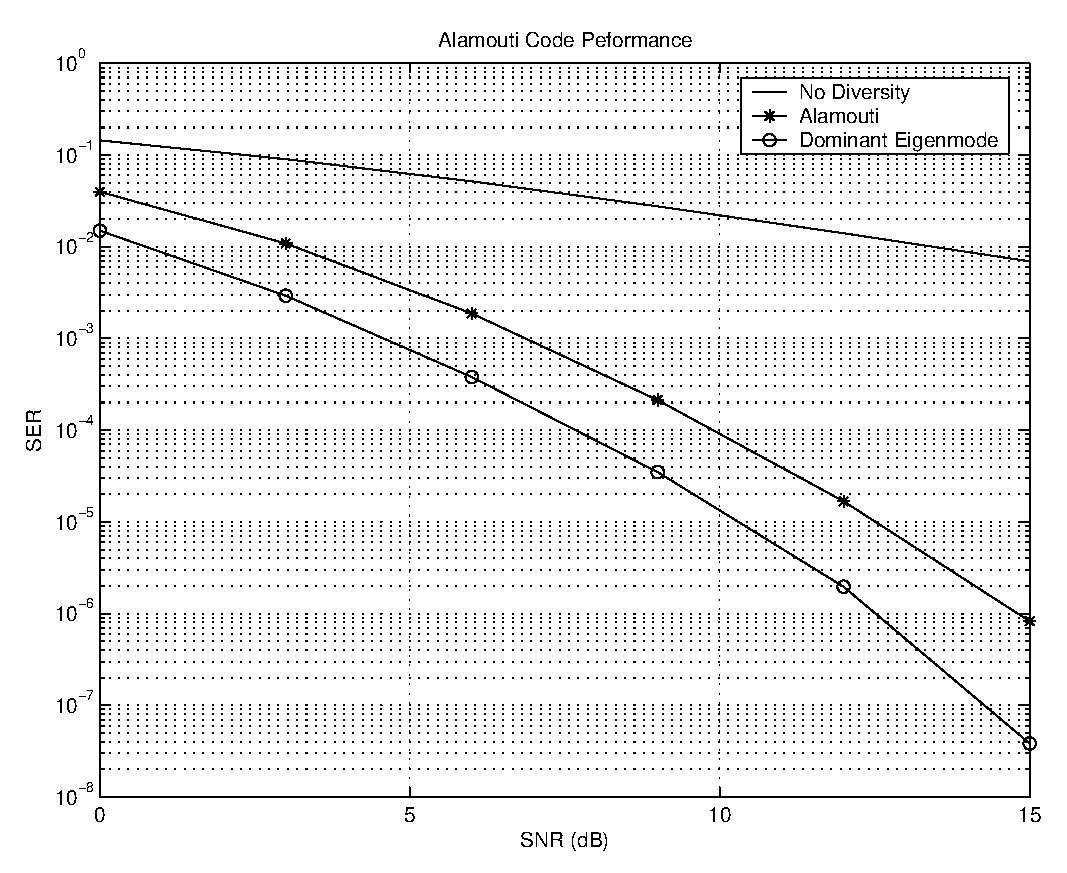
\includegraphics[width=0.7\columnwidth]{hw3_3.eps}
\end{center}
\begin{footnotesize}
\verbatiminput{ps3p3.m}
\end{footnotesize}
\end{enumerate}

\paragraph{Problem 5} \begin{enumerate}
\item The plots for ergodic and outage capacity are shown in Fig.
\ref{fig:p1_erg} and \ref{fig:p1_out}.  The pair of curves at the
bottom of each plot is for the case of a 2$\times$2 system.  The
other pairs going up correspond to increasing number of antennas.
At low SNR values the channel capacity improves dramatically with
channel knowledge.  Channel knowledge becomes less and less
important as SNR increases.  The script follows:
\begin{footnotesize}
\verbatiminput{p1.m}
\verbatiminput{pwr_modes.m}
\end{footnotesize}
%You can find this script as well as the pwr\_modes function on the web.
\begin{figure}
  % Requires \usepackage{graphicx}
  \centering
  \includegraphics[width=4in]{p1c_vs_snr.eps}\\
  \caption{\footnotesize Ergodic capacity vs SNR.  Channel known (dotted line) and channel unknown(solid line)}
  \label{fig:p1_erg}
\end{figure}
\begin{figure}
  \centering
  % Requires \usepackage{graphicx}
  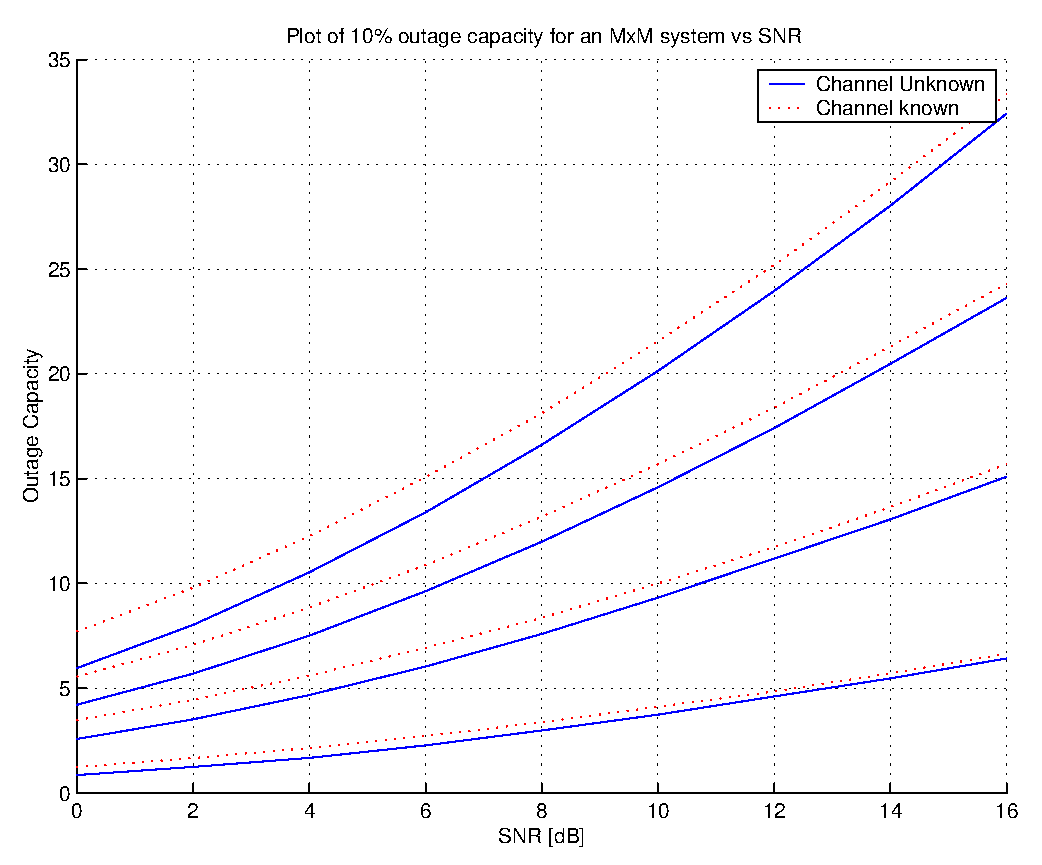
\includegraphics[width=4in]{p1c_outage_vs_snr.eps}\\
  \caption{\footnotesize 10\% outage capacity vs SNR.  Channel known (dotted line) and channel unknown(solid line)}
  \label{fig:p1_out}
\end{figure}

\item Fig \ref{fig:p1_erg_ant} shows the ergodic capacity as a function
of the number of antennas, $M$, at 10~dB SNR.  Here, channel
knowledge becomes more important for increasing $M$.  This is
because there are more modes in the channel if there are more
antennas. Thus the gain with waterfilling increases.
\begin{figure}
  % Requires \usepackage{graphicx}
  \centering
  \includegraphics[width=4in]{p1c_vs_ntx.eps}\\
  \caption{\footnotesize Ergodic capacity vs number of antennas.
  Channel known (dotted line) and channel unknown(solid line)}
  \label{fig:p1_erg_ant}
\end{figure}
\end{enumerate}

\end{document}

















